%%%%%%%%%%%%%%%%%%%%%%%%%%%%%%%%%%%%%%%%%%%%%%%%%%%%%%%%%%%%%%%%%%%%%%%%%%%%%%%%%
%																				%
%			Elen4016-Final-Report.tex			%
%																				%
% Ntsako Manyike (28 April 2011)							%
%																				%
% 				%
%														%
% %
% Note: Minor modifications were made to the original paper %
% by KJ Nixon 2005/10/12 (with permission from the original author %
%																				%
%%%%%%%%%%%%%%%%%%%%%%%%%%%%%%%%%%%%%%%%%%%%%%%%%%%%%%%%%%%%%%%%%%%%%%%%%%%%%%%%%

\documentclass[10pt,twocolumn]{witseiepaper}

%
% All KJN's macros and goodies (some shameless borrowing from SPL)
\usepackage{KJN}
\usepackage{rotating}
\usepackage{graphicx}
\usepackage{caption}
\usepackage{amsmath}

%
% PDF Info
%
\ifpdf
\pdfinfo{
/Title (Active suspension modelling and control)
/Author (Ntsako Kennedy Manyike)
/CreationDate (D:2011041700)
/ModDate (D:200410220900)
/Subject (Final Report)
/Keywords (ABS,)
}
\fi

%%%%%%%%%%%%%%%%%%%%%%%%%%%%%%%%%%%%%%%%%%%%%%%%%%%%%%%%%%%%%%%%%%%%%%%%%%%%%%%
\begin{document}


\title{ELEN4016 (LABORATORY): ACTIVE SUSPENSION MODELLING AND CONTROL}

\author{Ntsako Manyike}

\thanks{School of Electrical \& Information Engineering, University of the
Witwatersrand, Private Bag 3, 2050, Johannesburg, South Africa}



%%%%%%%%%%%%%%%%%%%%%%%%%%%%%%%%%%%%%%%%%%%%%%%%%%%%%%%%%%%%%%%%%%%%%%%%%%%%%%%
%
\abstract{To develop a robust controller that can improve the performances of the nonlinear active suspension system and its verifications using graphical and animation output. A stepwise approach with successive refinements of model and controller is undertaken. To develop a nonlinear mathematical model of the active suspension system for a quarter car model. To develop the control algorithm that based on a robust control scheme for the active suspension system.}

\keywords{Active actuator, Suspension travel, ABS, Feedback, State-space}


\maketitle
\thispagestyle{empty}\pagestyle{empty}


%%%%%%%%%%%%%%%%%%%%%%%%%%%%%%%%%%%%%%%%%%%%%%%%%%%%%%%%%%%%%%%%%%%%%%%%%%%%%%%
%
\section{INTRODUCTION}

Demands for better ride comfort and controllability of road vehicles are pursued by many in the car manufacturing industry. The purpose of a car suspension is to improve the ride comfort for passengers and to improve car handling. Suspension is the term given to the system of springs, shock absorbers and linkages that connects a vehicle to its wheels \cite{Ghita:2008}. Ride comfort can be classified as the body acceleration attenuation during driving when the road profile changes, sprung mass vertical displacement peaks reduction i.e minimizing the vertical car body acceleration. Car handling can be characterized as vehicle stability and controllability reduction during braking, accelerating and driving through curves and tire jumping.

In any car suspension system, there are a variety of performance parameters which need to be optimized. The trade-off between ride comfort and handling characteristics is usually a trial and error procedure which represents an optimization problem. There are four important parameters which should be considered carefully in designing a suspension system: namely, ride comfort, body motion, road handling and suspension travel.

No suspension system can simultaneously minimize all four of the above mentioned parameters \cite{Taghirad:1995}. On most cars the emphasis on suspension design is on comfort and adequate safety which is in contrast to a sports-car suspension where the emphasis is on safety with comfort only being a minor consideration. A design conflict exists between a suspension that should be soft to minimise acceleration levels and one that is hard to maintain good tyre-ground contact. It is important for the suspension to keep the road wheel in contact with the road surface as much as possible. The suspension also protects the vehicle itself and any cargo or luggage from damage and wear. Finding right compromise between these conflicting requirements has been the problem with classical passive suspension design.

To satisfy all of these above mentioned requirements, it is necessary to change damping characteristic of the suspension system dynamically with respect to the road situation. Active suspension control is concerned with controlling the vertical movements of the vehicle in response to the fast changing road surface properties. The advantage of controlled active suspension is that a better set of design trade-offs are possible rather than with passive systems. An active car suspension design allows car manufacturers to achieve a higher degree of both ride quality and car handling by keeping the tires perpendicular to the road in corners, allowing for much higher levels of grip and control.

The project involves the development of a controller for a quarter car system suspension. This model is investigated to determine whether the suspension travel or the suspension dynamic force is the most suitable output for incorporation with the ABS for improved braking control. State-feedback control for active suspension is a powerful tool for designing a controller. In this approach a mathematical representation for ride comfort and road handling will be optimized considering the actuator limitations. Since body motion and suspension travel are functions of the system states, they will also be optimized during the design.

%%%%%%%%%%%%%%%%%%%%%%%%%%%%%%%%%%%%%%%%%%%%%%%%%%%%%%%%%%%%%%%%%%%%%%%%%%%%%%%%
\section{BACKGROUND}

A car suspension system is the mechanism that physically separates the car body from the wheels of the car. The performance of the suspension system has been greatly increased due to increasing vehicle capabilities. One of the performance requirements in advanced suspension systems which prevent the road disturbances to affect the passenger comfort associated with cornering and braking or acceleration while increasing riding capabilities and performing a smooth drive \cite{Ghita:2008}. 

The use of active suspension on road vehicles has been considered for many years \cite{Thompson:1970}, and a large number of different arrangements from semi-active to fully active schemes have been investigated \cite{Sharp:1987}. Typically there are three suspension structures, passive suspension, semi-active suspension and active suspension system according to external power input to the system.

%%%%%%%%%%%%%%%%%%%%%%%%%%%%%%%%%%%%%%%%%%%%%%%%%%%%%%%%%%%%%%%%%%%%%%%%%%%%%%%%
\subsection{Passive suspension system} 

A passive suspension system consists of traditional springs and shock-absorbing dampers. The suspension system can only control the motion of the car body and wheel by limiting the suspension velocity according to the rate determined by the designer. The fixed characteristics depend on the environment where suspension is deployed. Passive suspension design is a compromise between comfortable ride and vehicle handling \cite{Williams:1994}. Heavy damping yields good vehicle stability but most of the road bumps are transferred to the body. Hence ride is not enjoyable to the passanger and cargo might be damaged. Lightly damped suspension will improve comfort but reduces stability especially in turns.

The suspension spring and damper do not provide energy to the suspension system and control only the motion of the car body and wheel by limiting the suspension velocity according to a fixed rate \cite{Wright:1984}. Hence, the performance of a passive suspension system is variable subject to the road profiles. It's advantages are that is it low-cost and simple. The fixed linear spring and damper limit the dynamic response of this system.

%%%%%%%%%%%%%%%%%%%%%%%%%%%%%%%%%%%%%%%%%%%%%%%%%%%%%%%%%%%%%%%%%%%%%%%%%%%%%%%%
\subsection{Semi-active suspension system} 

The semi-active suspension has the same elements but the damper has two or more selectable damping rate. Two types of dampers are used in the semi-active suspension namely the two state dampers and the continuous variable dampers \cite{Donahue:1998}. The disadvantage of these dampers is difficulties to find devices that are capable in generating a high force at low velocities and a low force at high velocities, and be able to move rapidly between the two. 

The damper requires additional power and can not generate an independent force from the system. It is also more complex and more expensive than the passive suspension system.

%%%%%%%%%%%%%%%%%%%%%%%%%%%%%%%%%%%%%%%%%%%%%%%%%%%%%%%%%%%%%%%%%%%%%%%%%%%%%%%%
\subsection{Active suspension system} 

The active suspension system which is being studied here has an active actuator between the chasis and the car body. An active actuator is a device used to convert an electrical signal to mechanical motion. The active actuation can be accomplished using a variety of components. Some examples include electromechanical actuators, hydraulic actuators, and pneumatic actuators. In the latest brake-by-wire systems, electro-machanic actuators are used \cite{Ghita:2008}. These are capable of delivering continously varying and different brake force on each wheel. Each system has its own distinct strengths such as response time and power requirements. The suspension actuators are implemented simply as controllable force inputs. The physical method of force actuation is not discussed in this paper. This will allow more flexibility once the control system has been designed for selecting the most appropriate actuator based on the need of the system, i.e. power or response time. 

Active suspension can be devided into two categories: the low-bandwidth or soft active suspension and the high-bandwidth or stiff active suspension \cite{Crolla:1988}. Soft active suspensions are characterized by an actuator that is in series with a damper and the spring. Wheel hop motion is controlled passively by the damper, so that the active function of the suspension can be restricted to body motion. Therefore, such type of suspension can only improve the ride comfort. A high-bandwidth or stiff active suspension is characterized by an actuator placed in parallel with the damper and the spring as illustrated in ~\figref{fig:system}. This is the suspension system that is under investigation in this study. Since the actuator connects the unsprung mass to the body, it can control both the wheel hop motion as well as the body motion \cite{Williams:1994, Wright:1984} i.e. requirements mentioned above. Thus the active suspension can improve both the ride comfort and handling simultaneously. The additional power requirement for the actuator is one of the disadvantages of the active suspension system. 

%%%%%%%%%%%%%%%%%%%%%%%%%%%%%%%%%%%%%%%%%%%%%%%%%%%%%%%%%%%%%%%%%%%%%%%%%%%%%%%
\section{MODELLING} 
The mathematical model of the suspension system. An initial simplifying assumption is that the suspension is linear, after a suspension model is obtained, the non-linear characteristics of the suspension system are incoperated into the model.

%%%%%%%%%%%%%%%%%%%%%%%%%%%%%%%%%%%%%%%%%%%%%%%%%%%%%%%%%%%%%%%%%%%%%%%%%%%%%%%
\subsection{System overview}

The studies of active suspension system have been performed using various suspension models. The quarter car model is the model that will be investigated. Other suspension models are the half and the full car body models. These control design models are not used because the models is highly non-linear, thus the known algorithms from control design like pole placement or quadratic linear regulator require a lot of math to realise the models. The number of degrees of freedom also usually exceeds 50 resulting in large computational requirements which are out of scope for this project \cite{Sharp:1987}. In the quarter car model, only the interaction between the quarter car body and the single wheel is considered.

The quarter car model is the fundamental model which can provide basic information regarding brake system behaviour which is the goal of the laboratory. Motion of the car is only in the vertical direction. ~\figref{fig:system} shows the quarter car set up with the nomenclature used. 

The objective of the model created was to assist in the development of a control system for the vehicle’s active suspension system. A high level of detail could have been included in the development of the model, however assumptions were made to simplify the model. These simplifications help remove unnecessary details that are not of interest when optimizing the vertical dynamics of the vehicle. The assumptions also help reduce the computational requirements of the simulation. The following assumptions are made with regards to the model:
\begin{itemize}
	\item The body of the vehicle is rigid.
	\item The tire is modeled as a single linear spring.
	\item The suspension damper and spring are linear.
	\item The active actuator is linear.
	\item The lateral and longitudinal motion of the tires is negligible compared to their vertical motion.
	\item The vehicle is not skidding.
\end{itemize}

The last two assumptions are essential for when the system is integrated with the ABS model.
 
\begin{figure}[ht]
	\centering
		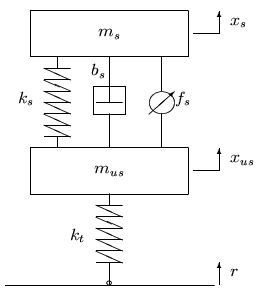
\includegraphics[width=0.25\textwidth]{QuarterCarModel.jpg}
	\caption{ Active Suspension for Quarter Car Model}
	\label{fig:system}
\end{figure}

The model consists of the sprung mass (car chassis), $\textit{m}_{s}$, and the unsprung mass (wheel assembly), $\textit{m}_{us}$, respectively, $\textit{k}_{s}$ and $\textit{k}_{t}$ are the stiffness of the car body spring and car tyre, respectively, $\textit{b}_{s}$ is the damping constant for the damper, $\textit{x}_{s}$ and $\textit{k}_{u}$ are the vertical displacement of the car body and the car wheel, respectively, $\textit{f}_{a}$ is the control force that generated by the active actuator and $\textit{r}$ is an irregular excitation from the road surface that may be considered negligible \cite{Nyandoro:2011}. 
%%Or alternately insert a table with the values

Applying Newton's laws of motion and Hook's law on the model in ~\figref{fig:system} results in the first order differential equations equations ~\ref{eqn:xs} and ~\ref{eqn:xu}

\begin{equation}
	m_s \ddot{x_s} = -k_s(x_s - x_t) - b_s(\dot{x_s} - \dot{x_t}) - f_a
	\label{eqn:xs}
\end{equation}

\begin{equation}
	m_t \ddot{x_t} = k_s(x_s - x_t) - b_s(\dot{x_s} - \dot{x_t}) + f_a
	\label{eqn:xu}
\end{equation}

%%%%%%%%%%%%%%%%%%%%%%%%%%%%%%%%%%%%%%%%%%%%%%%%%%%%%%%%%%%%%%%%%%%%%%%%%%%%%%%
\subsection{State space model}

The linearity of this model permits the use of a statespace representation of the syste. By manipulating equations ~\ref{eqn:xs} and ~\ref{eqn:xu} the mathematical model of the active suspension system can be written in
state space form as:

\begin{array}{lcr}
	\mathbf{\mathit{\dot{x}}} & = & \mathbf{\mathit{Ax + Bu}} \\
	\mathbf{\mathit{y}} & = & \mathbf{\mathit{{Cx + Du}}
	\label{eqn:stateSpace}
\end{array}

%%%%%%%%%%%%%%%%%%%%%%%%%%%%%%%%%%%%%%%%%%%%%%%%%%%%%%%%%%%%%%%%%%%%%%%%%%%%%%%
\subsection{Active suspension with suspension travel as the reference input}
\begin{figure}[ht!]
	\centering
		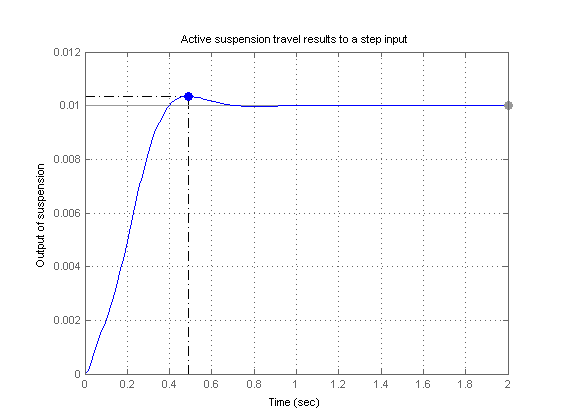
\includegraphics[width=0.50\textwidth]{suspention_travel.png}
	\caption{Quarter car active suspension response to suspension travel input}}
	\label{fig:force}
\end{figure}

The code to produce this results is listed below:

\begin{verbatim}
% mass of quarter car excluding wheel
ms = 427.0;    
% mass of wheel 
mw = 40.0;     
%spring constant for suspension  
Ks = 19960.0;  
% damper constant for suspension 
Cs = 1050.0;    
% spring constant for wheel
Kw = 175500.0;  

%state matrices
A = [0 1 0 0; 
-Ks/ms -Cs/ms Ks/ms Cs/ms; 
0 0 0 1; 
Ks/mw Cs/mw -(Ks+Kw)/mw -Cs/mw];
B = [0;
    -1/ms; 
    0; 
    1/mw];
C = [1 0 -1 0];
D = 0;

%check controllability
rank(ctrb(A,B));
%check observability
rank(obsv(A,C));

%It is required that the 
%system should s
%ettle in 0.5 seconds with an
%overshoot of less than 5 %
p1 = -35+15i;
p2 = -35-15i;
p3 = -9-7.75i;
p4 = -9+7.75i;
poles = [p1 p2 p3 p4];
 %Find the feddback gain matrix
Kgamma = place(A,B,poles)

%check controllability
Controllable = rank(ctrb(A,B));
%check observability
Observable = rank(obsv(A,C));

t = 0:0.01:2;
u = 0.01*ones(size(t));
Nbar=rscale(A,B,C,0,Kgamma)
lsim(A-B*Kgamma,B*Nbar,C,0,u,t)|
\end{verbatim}

%%%%%%%%%%%%%%%%%%%%%%%%%%%%%%%%%%%%%%%%%%%%%%%%%%%%%%%%%%%%%%%%%%%%%%%%%%%%%%% 
\subsection{Active suspension with suspension dynamic force as the reference input}

Using the Matlab function, place to calculate the closed loop pole position for a feedback regulator K, the \figref{fig:force} is realised.
\begin{figure}[h]
	\centering
		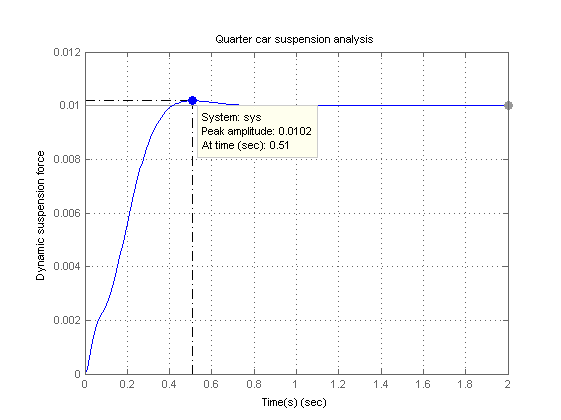
\includegraphics[width=0.50\textwidth]{Force_input.png}
	\caption{Quarter car active suspension response to active force input}}
	\label{fig:force}
\end{figure}

The code to plot the above graph is shown below:
\begin{verbatim}
	%Required parameters
% mass of quarter car excluding wheel
ms = 427.0;    
% mass of wheel 
mw = 40.0;     
%spring constant for suspension  
Ks = 19960.0;  
% damper constant for suspension 
Cs = 1050.0;    
% spring constant for wheel
Kw = 175500.0;  

%state matrices
A = [0 1 0 0; 
-Ks/ms -Cs/ms Ks/ms Cs/ms; 
0 0 0 1; 
Ks/mw Cs/mw -(Ks+Kw)/mw -Cs/mw];
B = [0;
    -1/ms; 
    0; 
    1/mw];
C = [0 0 1 0];
D = 0;

%check controllability
rank(ctrb(A,B));
%check observability
rank(obsv(A,C));

%It is required that the system 
%should settle in 0.5 seconds with an
%overshoot of less than 5 %
p1 = -20+5i;
p2 = -20-5i;
p3 = -8-10i;
p4 = -8+10i;
poles = [p1 p2 p3 p4];
%Find the feddback gain matrix
Krho = place(A,B,poles)

%check controllability
Controllable = rank(ctrb(A,B));
%check observability
Observable = rank(obsv(A,C));

t = 0:0.01:2;
u = 0.01*ones(size(t));
Nbar=rscale(A,B,C,0,Krho)
lsim(A-B*Krho,B*Nbar,C,0,u,t)
\end{verbatim}

%%%%%%%%%%%%%%%%%%%%%%%%%%%%%%%%%%%%%%%%%%%%%%%%%%%%%%%%%%%%%%%%%%%%%%%%%%%%%%%
\subsection{Controlability, observability and stability} 


Controllability was observed by determining the rank of the control matrix. See code for more information on this. Where B and A are the state space matrices and n is the number of states; 4 for  this model. It was observed that the system is controllable by using uncontrollable states in the system using the function  ctrb() in Matlab. 

Similarly, the Observability matrix was analyzed in Matlab using the C and A state space matrices (shown in Appendix C) and it was found that 8 states were unobservable. It was discovered that every state of the system was observable via the Cg roll angle, pitch angle, and vertical position. These three outputs would be produced in a physical vehicle by the integration of an accelerometer signal produced at the vehicle
Stability of the system was checked by determining the Eigen-values of the A matrix. All Eigen-values had a real component less than or equal to zero, and thus the system was deemed stable. 

%%%%%%%%%%%%%%%%%%%%%%%%%%%%%%%%%%%%%%%%%%%%%%%%%%%%%%%%%%%%%%%%%%%%%%%%%%%%%%%
\section{RESULTS AND ANALYSIS}

%%%%%%%%%%%%%%%%%%%%%%%%%%%%%%%%%%%%%%%%%%%%%%%%%%%%%%%%%%%%%%%%%%%%%%%%%%%%%%%%%
\section{CONCLUSION}

A quarter car model is used to realise an active suspension model in a state-space representation. Newton's laws of motion are applied to the quarter car system and the resulting linear differential equation is transformed to a state-space representation. A step input representing suspension travel is applied to the model and the results are plotted. This is repeated for a dynamic suspension force. This shows that state-space is a useful technique to use as a stepping stone for designing feedback controllers and such since one can see each state of the system using software packages such as MATLAB.

%%%%%%%%%%%%%%%%%%%%%%%%%%%%%%%%%%%%%%%%%%%%%%%%%%%%%%%%%%%%%%%%%%%%%%%%%%%%%%%%%


\bibliographystyle{witseie}
\bibliography{references}

%%%%%%%%%%%%%%%%%%%%%%%%%%%%%%%%%%%%%%%%%%%%%%%%%%%%%%%%%%%%%%%%%%%%%%%%%%%%%%%


%{\tiny \vfill \hfill \today \hspace{5mm} witseie-paper-2003.\TeX}

\end{document}

" vim: ts=4
" vim: tw=78
" vim: autoindent
" vim: shiftwidth=4

